\chapter{Synthèse et optimisation des circuits séquentiels}
\section{Classes et représentation}
Rappelons que l'état du système n'est pas forcement visible par l'extérieur.\\
La sortie d'un système est fonction de l'état et \textit{éventuellement} des entrées. Cet \textit{éventuellement} implique 2 classes de circuit logique séquentiel:
\begin{itemize}
	\item Machine de Moore (pas Gordon!)
	\item Machine de Meally
\end{itemize}
\paragraph{Machine de Moore:}
la \textbf{sortie} est \textbf{uniquement} fonction des \textbf{variables d'état}.
\begin{figure}[H]
	\centering
	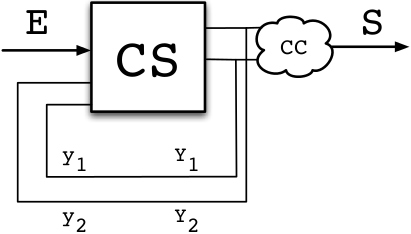
\includegraphics[width=.3\textwidth]{ch7/image1}
\end{figure}
\paragraph{Machine de Meally:}
la \textbf{sortie} est fonction (combinatoire) des \textbf{variables d'état} et des \textbf{entrées}.
\begin{figure}[H]
	\centering
	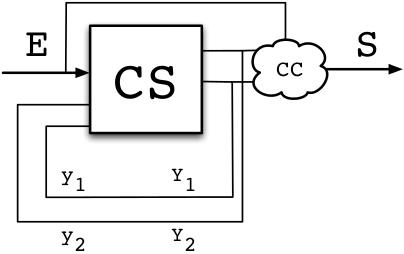
\includegraphics[width=.3\textwidth]{ch7/image2}
\end{figure}

Pour la synthèse à partir d'un cahier de charges verbal :
\begin{enumerate}
	\item Table d'état (ou Table de Huffman)
	\item Graphe d'état (optionnel)
	\item Équations logiques (et le circuit logique)
\end{enumerate}
\subsection{Codage des états}
On souhaite représenter les systèmes séquentiels à l'aide des codes binaires $\{0, 1, \text{-}\}$. Ce processus d'attribution de codes binaires aux états codés s'appelle \textit{le codage des états}.\\
Le nombre de bits nécessaires pour coder $n$ états est donné par $\log_2n$.
\subsubsection{Exemple}
Soit un système à 4 états. Attribuons à chaque état un code binaire (4 états $\rightarrow \log_2 4=2\rightarrow$ 2 bits nécessaires).\\
Ainsi $1\rightarrow 00,\ 2\rightarrow 01,\ 3\rightarrow 11,\ 4\rightarrow 10$.\\
Ainsi, on obtient:
\begin{figure}[H]
	\centering
	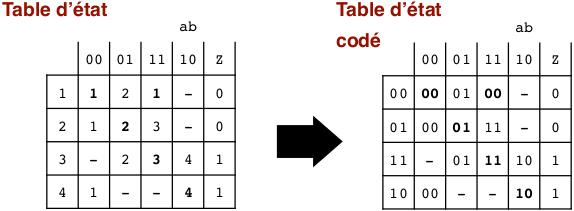
\includegraphics[width=.6\textwidth]{ch7/image3}
\end{figure}
À chaque bit du code correspond une fonction logique. On a donc : 4 états et 2 variables d'états ($y_2y_1$)$\rightarrow$ 2 fonctions logiques.
\begin{figure}[H]
	\centering
	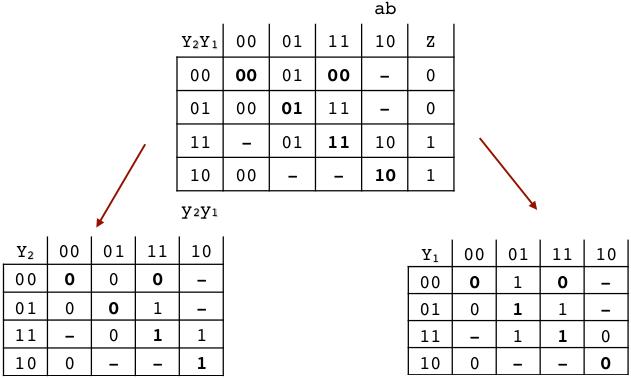
\includegraphics[width=.7\textwidth]{ch7/image4}
\end{figure}
Il suffit de simplifier la K-Map de $Y_2$ et celle de $Y_1$ et déduire leur fonction logique respective
\begin{figure}[H]
	\centering
	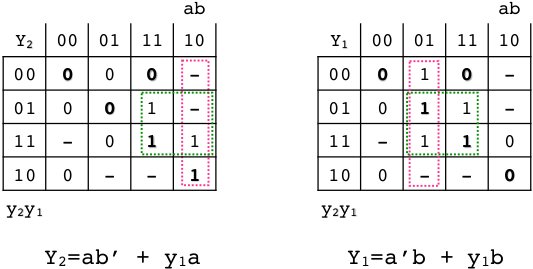
\includegraphics[width=.7\textwidth]{ch7/image5}
\end{figure}
\danger $y_2y_1\neq Y_2Y_1$, les premières représentent le présent, les 2 autres le futur.\\

Établissons la \textit{fonction de sortie}. Connaissant la valeur de sortie des états stables, nous pouvons remplir les cases correspondantes.
\begin{figure}[H]
	\centering
	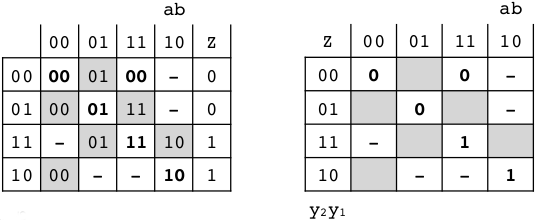
\includegraphics[width=.7\textwidth]{ch7/image6}
\end{figure} Pour les transitions (cases grises), il faut respecter les transitions ainsi que la règle suivante:
\begin{center}
	\textbf{Lors des transitions, si la sortie doit changer, elle ne devrait changer qu'une seule fois}
\end{center}
c-à-d que les \textbf{seules} possibilités sont
\begin{figure}[H]
	\centering
	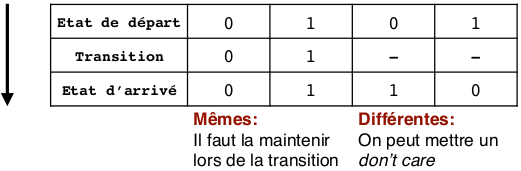
\includegraphics[width=.7\textwidth]{ch7/image7}
\end{figure}
Nous obtenons donc
\begin{figure}[H]
	\centering
	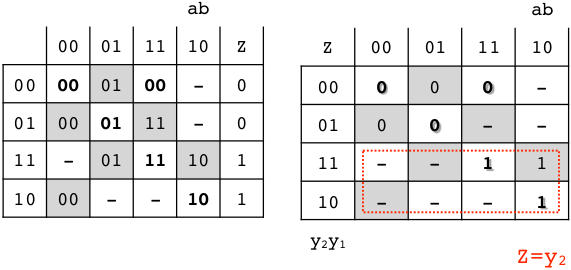
\includegraphics[width=.7\textwidth]{ch7/image8}
\end{figure}
Le logigramme correspondant n'est autre que
\begin{figure}[H]
	\centering
	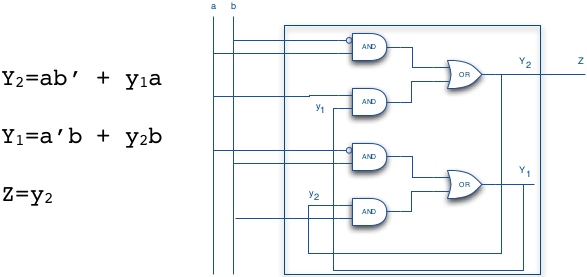
\includegraphics[width=.8\textwidth]{ch7/image9}
\end{figure}
\section{Simplification de la table primitive des états}
L’algorithme de synthèse se constitue de 3 étapes :
\begin{enumerate}
	\item Table primitive d'état ou Table de Huffman :
	\begin{itemize}
		\item Écrire la table de Huffman à partir d'un cahier de charges.
		\item La \textbf{1\up{ère}} table ne peut avoir qu'\textbf{un seul état stable par ligne de la table d'état}
	\end{itemize}
	\item Codage des états
	\item Équations logiques
\end{enumerate}
La complexité du circuit obtenu lors de la synthèse est influencé par la complexité (taille) de la taille initiale d'état.\\
Chaque bit de code ($\log_2n$ bits de code pour $n$ états) représente:
\begin{itemize}
	\item une fonction logique
	\item un organe de mémoire (délais)
\end{itemize}
Il faut donc réduire le nombre d'états pour simplifier le circuit correspondant.
\subsection{Réduction du nombre d'état}
\subsubsection{Notion d'équivalence de deux états}
Deux états sont équivalents si (équivalence de deux états stables):
\begin{enumerate}
	\item ils produisent la \textbf{même sortie}
	\item pour \textbf{toutes} combinaisons des variables d'entrée, les \textbf{futurs} états sont soit les mêmes soit \textbf{équivalents}
\end{enumerate}
Nous obtenons donc deux types d'équivalence:
\begin{itemize}
	\item \textbf{États identique} : 2 (ou plus) états stables sont au même endroit (même combinaison des entrées)
	\begin{figure}[H]
		\centering
		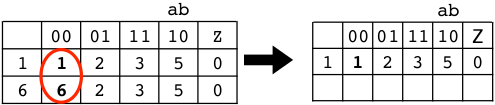
\includegraphics[width=.7\textwidth]{ch7/image10}
	\end{figure}
	\item \textbf{États fusionnables} : les états stables se trouvent à des endroits différents (combinaison des entrées différentes)
	\begin{figure}[H]
		\centering
		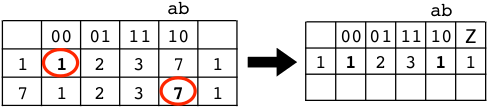
\includegraphics[width=.7\textwidth]{ch7/image11}
	\end{figure}
\end{itemize}
Pour que $n$-états soient équivalents il faut que tous les états soient équivalents deux à deux.\\

Pour ce faire, on dresse un tableau de $n(n-1)/2$ cases appelé \textbf{table des conditions d'équivalences}:
\begin{itemize}
	\item Chaque case de la table représente la possibilité d'équivalence et/ou de fusionnement de deux états
	\item \textbf{Dans le cas de la machine de Moore}, toute paire d'états ayant la sortie différente peut être exclue
	\item L'impossibilité de fusionner deux états se note par une croix
\end{itemize}
Pour 11 états, la table des conditions d'équivalence ressemble à:
\begin{figure}[H]
	\centering
	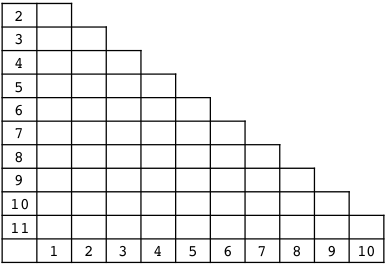
\includegraphics[width=.6\textwidth]{ch7/image12}
\end{figure}
\section{Synthèse d'un flip-flop D}
\begin{wrapfigure}{r}{.5\textwidth}
	\centering
	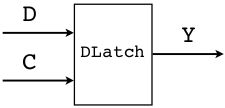
\includegraphics[width=.3\textwidth]{ch7/image13}
\end{wrapfigure}
\subsection{D-Latch:} Mémoire suiveuse-bloqueuse (\textit{Sample and Hold}).\\
Spécification:
\begin{itemize}
	\item 2 entrées : D (\textit{data}) et C (\textit{control})
	\item Une sortie : Y
	\item La sortie prend la valeur de l'entrée D lorsque C$=1$
\end{itemize}
\subsection{Flip-flop D (\textit{edge triggered})}
\label{subsec:Dflipflop}
\begin{wrapfigure}{r}{.5\textwidth}
	\centering
	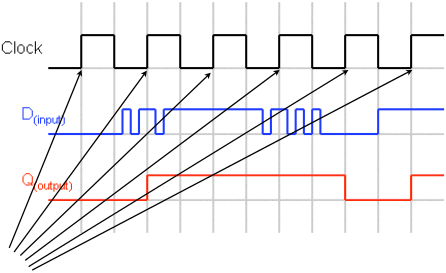
\includegraphics[width=.4\textwidth]{ch7/image14}
\end{wrapfigure}
Spécification :
\begin{itemize}
	\item La sortie prend la valeur de D \textbf{uniquement} lors d'un \textbf{flanc montant} de C (passage de $0\rightarrow 1$)
	\item Entre 2 flancs montants, la valeur de D est maintenue (toute variation de D est ignorée)
	\item Si C est sur un flanc montant et que D varie, la sortie prend l'ancienne valeur de D, celle juste avant le flanc montant 
	\item Le reste n'est que maintient
\end{itemize}
\subsubsection{Table primitive d'état}
\begin{minipage}{.5\textwidth}
	Considérons l'évolution qui mettra la sortie à 1:
\begin{enumerate}
	\item Situation de départ $\rightarrow Q=0$ et aucun changement à l'entrée (le $CD=00$ ne change pas) $\Rightarrow$ état 1
	\item $D$ change ($0\rightarrow 1$) avant $C$ $\Rightarrow$ état 2
	\item $C$ change $\Rightarrow$ état 4
\end{enumerate}
\end{minipage}
\vspace{-2.9cm}
\begin{minipage}{.5\textwidth}
	\begin{figure}[H]
		\centering
		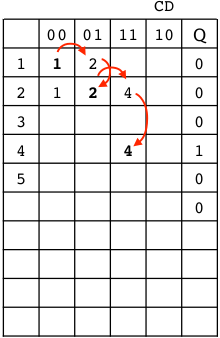
\includegraphics[width=.7\textwidth]{ch7/image15}
	\end{figure}
\end{minipage}
\begin{minipage}{.5\textwidth}
	Considérons maintenant une autre évolution en partant de l'état 1
	\begin{enumerate}
		\item $C$ change avant $D$ ($CD=00\rightarrow 10$) $\Rightarrow$ état 3
		\item $D$ change, le système ignore sa variation $\Rightarrow$ état 5 (diffère de l'état 4 par la valeur de la sortie $Q$)
	\end{enumerate}
\end{minipage}
\begin{minipage}{.5\textwidth}
	\begin{figure}[H]
		\centering
		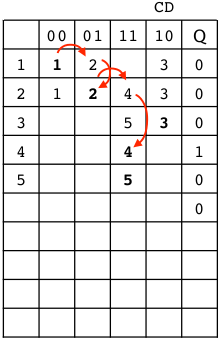
\includegraphics[width=.7\textwidth]{ch7/image16}
	\end{figure}
\end{minipage}

\begin{minipage}{.5\textwidth}
	Principe de mémorisation d'un 1
	\begin{enumerate}
		\item Initialement : $CD=00$
		\item $CD=00\rightarrow 01\rightarrow 11$
		\item $Q=0\rightarrow 1$ (état 4)
		\item $C=0 \Rightarrow$ peu importe la valeur de $D$, la sortie reste à 1 (états 7 et 9)
	\end{enumerate}
\end{minipage}
\begin{minipage}{.5\textwidth}
	\begin{figure}[H]
		\centering
		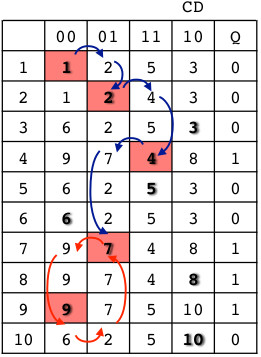
\includegraphics[width=.7\textwidth]{ch7/image17}
	\end{figure}
\end{minipage}

\subsubsection{Table de conditions d'équivalences}
Cette table se définit en 3 passes:
\begin{enumerate}
	\item[-- Passe 1.] Sorties différentes
	\begin{figure}[H]
		\centering
		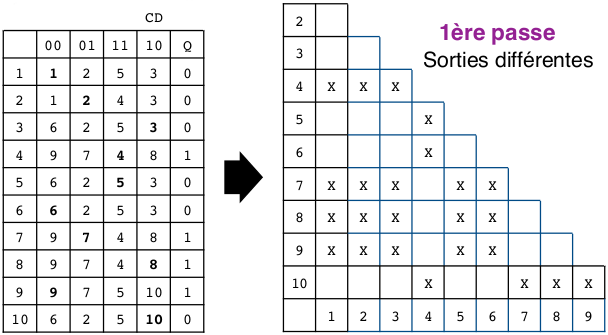
\includegraphics[width=.7\textwidth]{ch7/image18}
	\end{figure}
	\item[-- Passe 2.] Conditions de fusionnements 
	\begin{figure}[H]
		\centering
		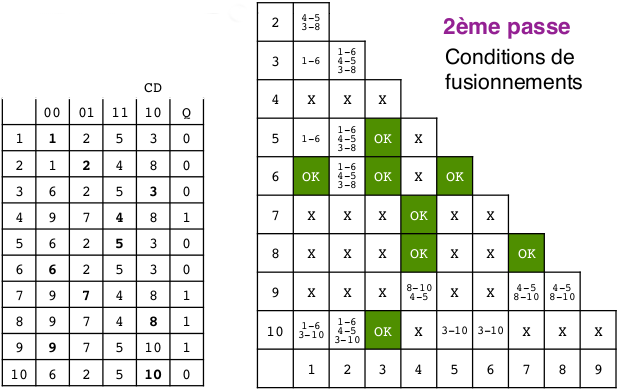
\includegraphics[width=.7\textwidth]{ch7/image19}
	\end{figure}
	\item[-- Passe 3.] Suppression des impossibles
	\begin{figure}[H]
		\centering
		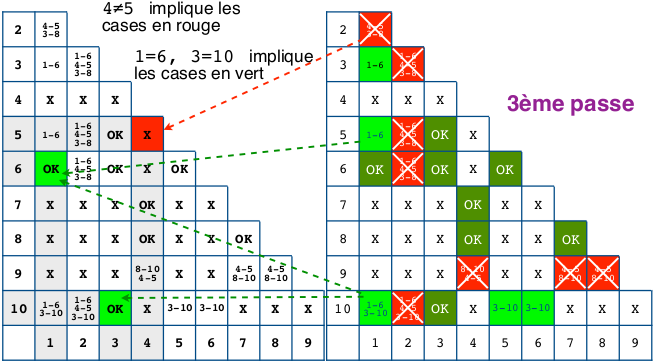
\includegraphics[width=.7\textwidth]{ch7/image20}
	\end{figure}
\end{enumerate}
Nous pouvons donc obtenir de ce tableau une liste assez claire des fusionnements possibles :
\begin{figure}[H]
	\centering
	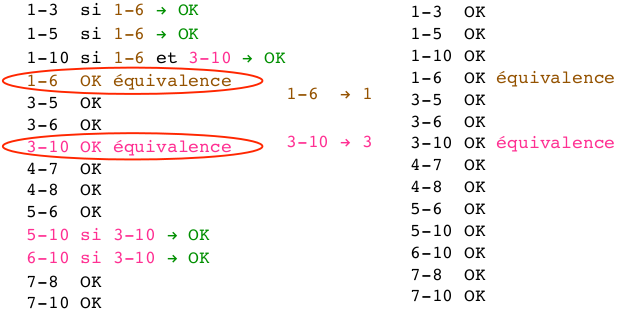
\includegraphics[width=.7\textwidth]{ch7/image21}
\end{figure}
Après avoir établi nos choix de fusionnement, il suffit de les appliquer à la table primitive d'état et de réordonner pour plus de lisibilité :
\begin{figure}[H]
	\centering
	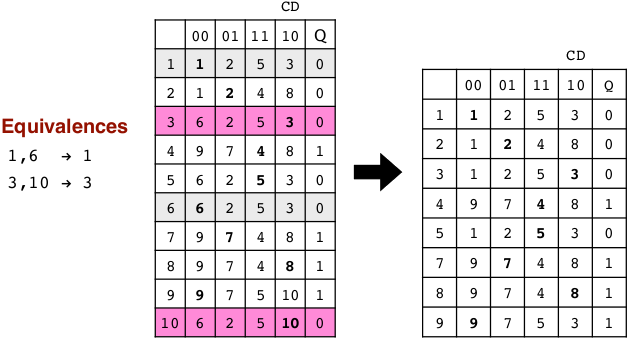
\includegraphics[width=.7\textwidth]{ch7/image22}
\end{figure}
\begin{figure}[H]
	\centering
	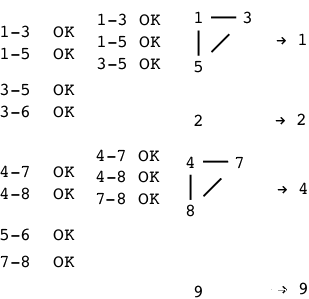
\includegraphics[width=.4\textwidth]{ch7/image22bis}
\end{figure}
\begin{figure}[H]
	\centering
	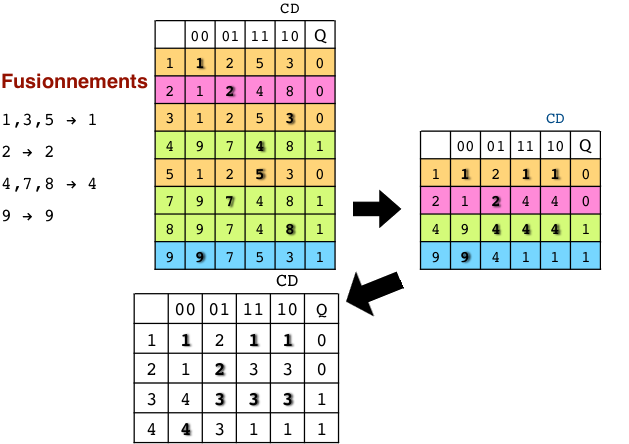
\includegraphics[width=.7\textwidth]{ch7/image22bisbis}
\end{figure}

Nous passons donc de 10 à 4 états $\Rightarrow$ 2 variables d'état au lieu de 4 !\\

Le choix du codage des états étant (pour l'instant) arbitraire : $1\rightarrow 00,\ 2\rightarrow 01,\ 3\rightarrow 11,\ 4\rightarrow 10$. Il ne reste plus qu'à écrire la K-Map de chaque variable d'état et d'en déduire leur fonction logique:
 \begin{figure}[H]
 	\centering
 	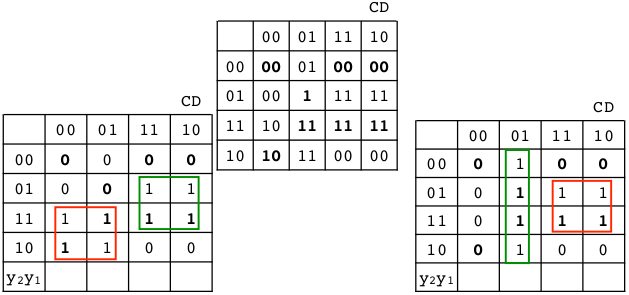
\includegraphics[width=.7\textwidth]{ch7/image23}
 \end{figure}
\section{Différents organes de mémoire}
Nous verrons 4 type de flip-flop :
\begin{itemize}
	\item SR : $Q=1$ lorsque $S=1$. La combinaison $SR=11$ est interdite.
	\item JK : même chose que SR mais la combinaison interdite change d'état
	\item D : la sortie suit l'entrée
	\item T : changement d'état lorsque l'entrée $T=1$
\end{itemize}
\subsection{Description des flip-flops}
Nous verrons 3 manières pour décrire un flip-flop :
\begin{itemize}
	\item Table de fonctionnement (sorte de table d'état)
	\item Équations caractéristiques
	\item Table d'excitation 
\end{itemize}
On notera l'état présent par un Q et l'état futur par un Q\up{+}. À cela s'ajoute (pour la table d'excitation) 4 possibilités de couple présent-futur
\begin{figure}[H]
	\centering
	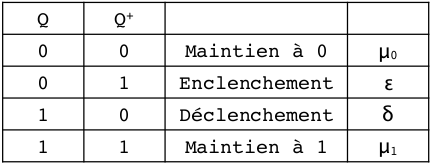
\includegraphics[width=.5\textwidth]{ch7/image24}
\end{figure}
\subsubsection{Flip-flop SR}
\begin{figure}[H]
	\centering
	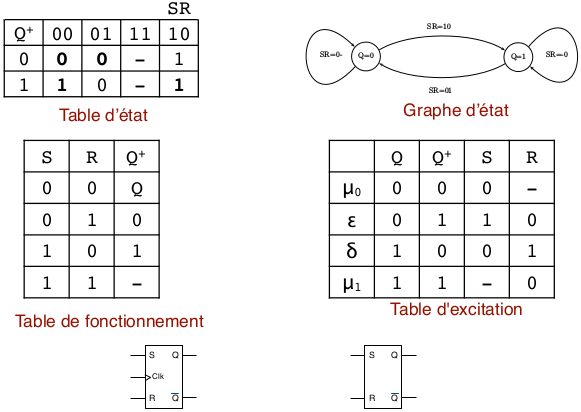
\includegraphics[width=.8\textwidth]{ch7/image25}
	\caption{Représentation schématique flip-flop SR}
\end{figure}
\subsubsection{Flip-flop JK}
\begin{figure}[H]
	\centering
	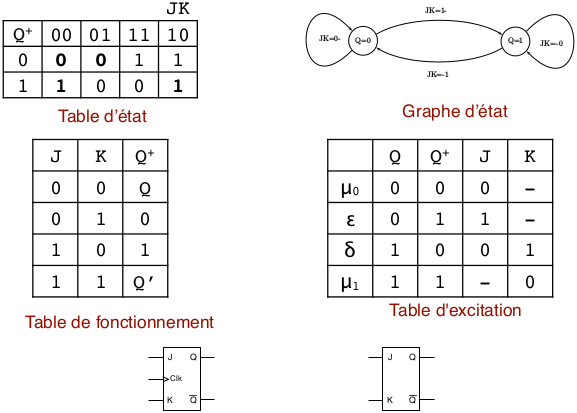
\includegraphics[width=.8\textwidth]{ch7/image26}
	\caption{Représentation schématique flip-flop JK}
\end{figure}
\subsubsection{Flip-flop D}
\begin{figure}[H]
	\centering
	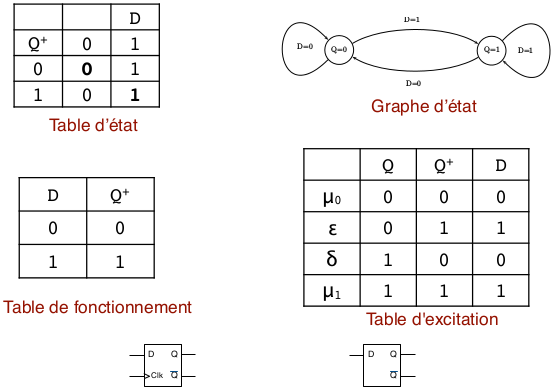
\includegraphics[width=.8\textwidth]{ch7/image27}
	\caption{Représentation schématique flip-flop D}
\end{figure}
\subsubsection{Flip-flop T}
\begin{figure}[H]
	\centering
	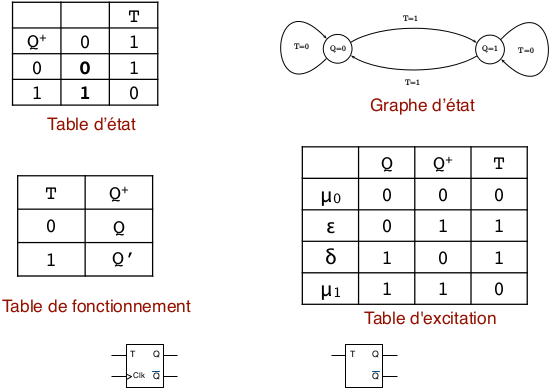
\includegraphics[width=.8\textwidth]{ch7/image28}
	\caption{Représentation schématique flip-flop T}
\end{figure}
\section{Courses critiques}
L'un des problèmes fondamental des circuits réels logiques à rétroaction est le problème des courses critiques. Il existe 2 méthodes de résolution des courses critiques 
\begin{itemize}
	\item Action sur le \textbf{codage des états} et les transitions $\Rightarrow$ conception des systèmes \textbf{séquentiels asynchrones}
	\item Action sur la \textbf{mise à jour} des variables d'état $\Rightarrow$ conception des systèmes \textbf{séquentiels synchrones}
\end{itemize}
\subsection{Origine du problème des courses critiques}
Prenons une table d'état déjà codée et faisons l'hypothèse que nous sommes dans l'état $00$ stable (c-à-d $ab=00$). Changeons les valeurs d'entrée $ab=00\rightarrow 11$. D'après la table, nous devons aller à l'état $11$. Nous avons donc $Y_1Y_2=00\rightarrow 11$. Regardons ce qu'il se passe en pratique
\begin{figure}[H]
	\centering
	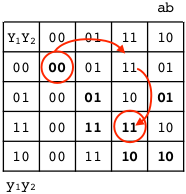
\includegraphics[width=.3\textwidth]{ch7/image29}
\end{figure}
\begin{figure}[H]
	\centering
	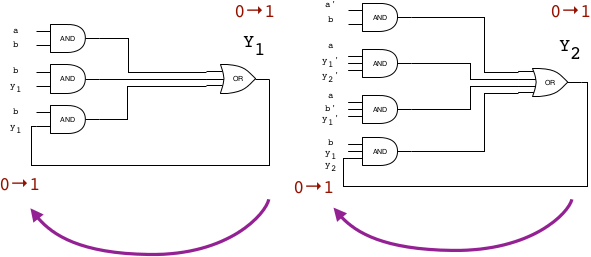
\includegraphics[width=.8\textwidth]{ch7/image30}
\end{figure}
Dans la boucle de rétroaction, la valeur de chacune des deux variables ($Y_1$ et $Y_2$) passe de $0$ à $1$. Or la transition dit $00\rightarrow 11$ donc le changement de valeur de chacune doit s'effectuer exactement en \emph{même temps} ! Si ces valeurs ne changent pas au même moment (fils de rétroaction de longueur différentes par exemple), il y a deux cas :
\begin{itemize}
	\item $Y_1$ a été plus vite que $Y_2$ ($Y_1Y_2=10$)
	\item $Y_2$ a été plus vite que $Y_1$ ($Y_1Y_2=01$)
\end{itemize} 
Donc au lieu de faire $00\rightarrow 11$ on fera $00\rightarrow 01\rightarrow ?$ ou  $00\rightarrow 10\rightarrow ?$. \emph{Le système présente un comportement non voulu (non-déterministe)}\dots
\begin{figure}[H]
	\centering
	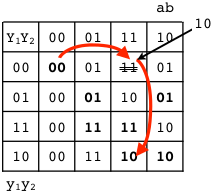
\includegraphics[width=.3\textwidth]{ch7/image31}
\end{figure}
Ainsi, les courses critiques se présenterons lorsque la distance de Hamming entre 2 états codées sera $>1$.
\subsection{Courses critiques et circuits logiques}
Il y a deux approches de résolutions des courses critiques :
\begin{itemize}
	\item on résout en les éliminant $\Rightarrow$ \emph{circuits asynchrones}
	\item on résout en synchronisant afin de mettre à jour le «futur» et ainsi attendre les variables d'états les plus lentes $\Rightarrow$ \emph{circuits synchrones} 
\end{itemize}

\paragraph{Remarque :} 
\begin{itemize}
	\item Ne pas confondre variables d'états et d'entrées
	\item Le changement des variables d'états n'a rien à voir avec le changement des entrées (les entrées sont des variables aléatoires)
	\item On considère que le changement simultané des variables d'entrées est possible
	\item On spécifie dans le cahier des charges le comportement du système dans le cas des variations simultanées des entrées
	\item Parfois, les variations simultanées sont impossibles (réservoir par exemple)
\end{itemize}
\begin{figure}[H]
	\centering
	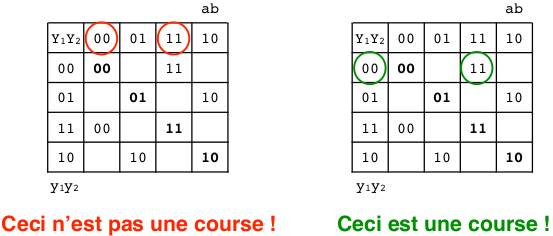
\includegraphics[width=.7\textwidth]{ch7/image32}
\end{figure}
\subsection{Méthodes de résolution des courses critiques pour des circuits asynchrones}
\label{subsec:resolcrit}
Il existe 3 méthodes, chacune devant être employée si la précédente n'a pas fonctionné (sauf la 1\up{ère} bien évidement), donc \emph{Méthode 1 $\rightarrow$ Méthode 2 $\rightarrow$ Méthode 3}\\
\danger On résout les courses (c-à-d en utilisant ces méthodes) uniquement pour le cas des systèmes asynchrones
\subsubsection{Méthode 1 : codage des états}
Cette méthode consiste à choisir un codage des états tels qu'il n'y ait pas de courses critiques (vu que le codage est arbitraire). Pour ce faire, on dessine un \emph{graphe de codage des états}, permettant de trouver le bon codage ou prouver qu'il n'en existe pas.
\paragraph{Graphe de codage des états :} un carré dont chaque sommet est un état stable, on représente les transitions (états futurs possibles pour chaque état) par un arc orienté. On attribue des codes et on réarrange de manière à ne plus avoir de courses critiques (distance d'Hamming de 1, arcs orientés formeront les arrêtes du carré). 
\begin{figure}[H]
	\centering
	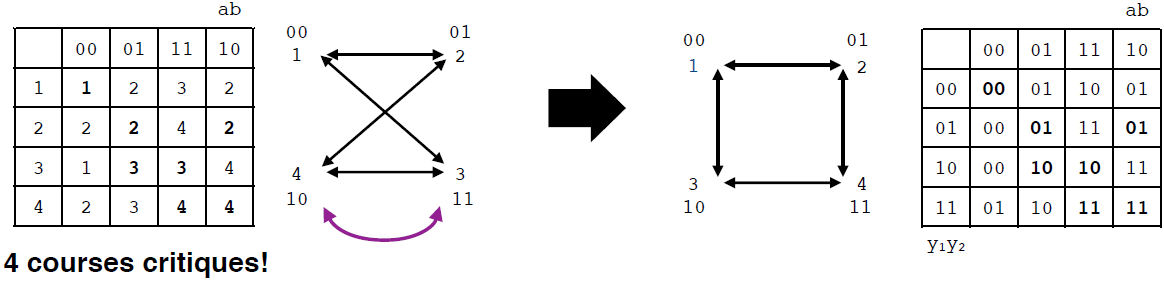
\includegraphics[width=\textwidth]{ch7/image33}
\end{figure}
Il faut néanmoins faire gaffe a switcher les lignes de tel manière a obtenir une K-map !
\begin{figure}[H]
	\centering
	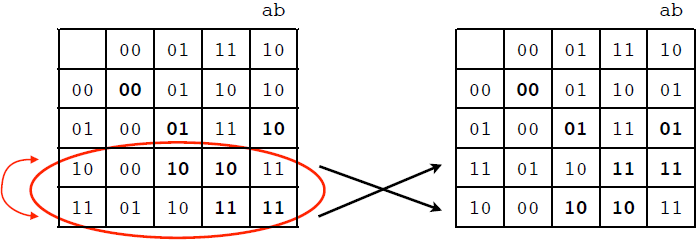
\includegraphics[width=.7\textwidth]{ch7/image34}
\end{figure}
On remarquera qu'il existe plusieurs combinaisons pour le codage des états, influençant la complexité du circuit (mais on ne doit pas en tenir compte :) ).\\
Il n'existe pas toujours une combinaison résolvant les courses critiques $\Rightarrow$ méthode 2
\begin{figure}[H]
	\centering
	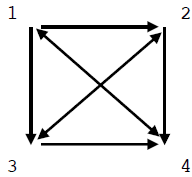
\includegraphics[width=.2\textwidth]{ch7/image35}
\end{figure}
\subsubsection{Méthode 2 : transitions}
On peut transformé une transition pour éviter la course critique (seul le point d'arrivé compte).
\begin{itemize}
	\item Utiliser les \textit{don't cares} :
	\begin{itemize}
		\item on transforme un \textit{don't care} en une transition pour éviter la course critique (par ex. $\textbf{1}\rightarrow 2\rightarrow 3\rightarrow \textbf{3}$)
	\end{itemize}
	\begin{figure}[H]
		\centering
		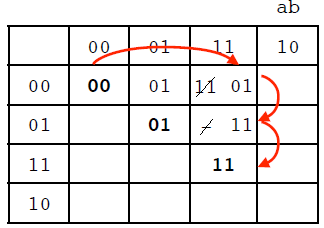
\includegraphics[width=.3\textwidth]{ch7/image36}
	\end{figure}
	\item Modifier les transitions :
	\begin{itemize}
		\item on utilise une transition déjà existante en passant par un autre état (par ex. $\textbf{1}\rightarrow 4\rightarrow 3\rightarrow \textbf{3}$)
	\end{itemize}
	\begin{figure}[H]
		\centering
		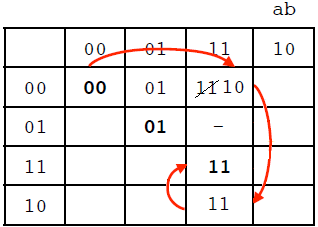
\includegraphics[width=.3\textwidth]{ch7/image37}
	\end{figure}
\end{itemize}
Les 2 sont bons !\\
Si ce n'est pas possible $\Rightarrow$ méthode 3
\subsubsection{Méthode 3 : état supplémentaire}
\textbf{Si et uniquement si} les 2 méthodes précédentes ont échouées, on rajoute une variable d'états (plutôt coûteux me direz-vous\dots) et on utilise ces nouveaux états comme intermédiaire de transition afin de résoudre les problèmes de courses.\\
Remarquons que toute course qui peut être résolue par les méthodes 1 et 2 avant, doit l'être.
\subsubsection{fautes graves}
\begin{enumerate}
	\item Laisser une course critique alors que l'on demande de faire la synthèse d'un circuit asynchrone.
	\item Ne pas appliquer les méthodes dans le bon ordre.
	\item dériver une K-map qui n'en est pas une (distance de Hamming $>1$ entre les lignes et les colonnes adjacentes).
\end{enumerate}
\section{Syntèses de la fonction de sortie}
\label{sec:synthfontsortie}
Toujours dans le cas de la machine de Moore, nous avons des problème de transitions pour la fonction de sorties (quelques glitchs).
\begin{figure}[H]
	\centering
	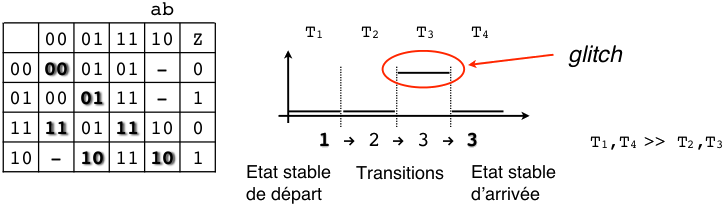
\includegraphics[width=.7\textwidth]{ch7/image38}
\end{figure}
Il faut donc réécrire la table de sortie pour toutes les transitions de la table d'état pour éviter les glitchs.

On commence par écrire les sorties des états stables (qui elles sont fixées) et les \textit{don't care} (donnant un \textit{don't care} en sortie). Passons aux transitions. 2 possibilités :
\begin{itemize}
	\item La valeur de départ et d'arriver est la même $\Rightarrow$ les transitions \textbf{doivent} garder la \textbf{même} valeur
	\begin{figure}[H]
		\centering
		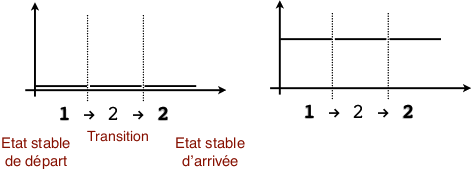
\includegraphics[width=.5\textwidth]{ch7/image39}
	\end{figure}
	\item La valeur de départ et d'arriver est différente $\Rightarrow$ il ne peut y avoir qu'\textbf{un seul} changement de la sortie (un \textit{don't care} et le reste fixé par l'état avant/après ce \textit{don't care})
		\begin{figure}[H]
			\centering
			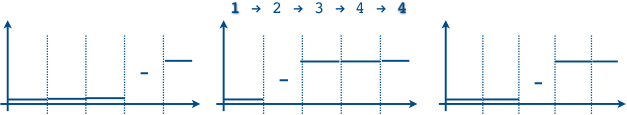
\includegraphics[width=.7\textwidth]{ch7/image40}
		\end{figure}
\end{itemize}
\danger une transition peut être utilisée pour le passage de différents états stables. Il faudra fixer la sortie de tel manière à satisfaire tous les passages
\begin{figure}[H]
	\centering
	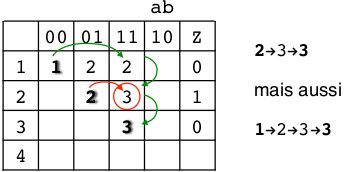
\includegraphics[width=.4\textwidth]{ch7/image41}
\end{figure}
Ainsi, nous obtenons
\begin{figure}[H]
	\centering
	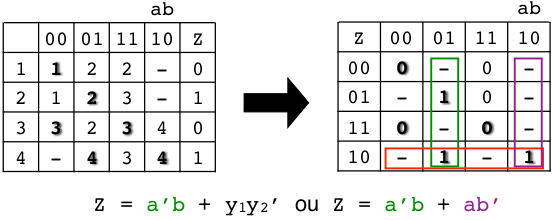
\includegraphics[width=.6\textwidth]{ch7/image42}
\end{figure}
\section{Machine de Meally}
La particularité de cette machine est que la sortie est fonction des variables d'état et des entrées.\\
\paragraph{Remarque :} Dans la machine de Moore, on a dû fixer les sorties des transitions pour éviter les glitchs. L'expression finale dépend de la sortie dépend des entrées, est-ce du coup une machine de Meally ? \textbf{NON}, la différence se fait lors des fusionnement des états.\\

Comme un même état stable peut avoir 2 sorties différentes, on note la sortie à coté de l'état stable (distingué par l'entrée)
\begin{figure}[H]
	\centering
	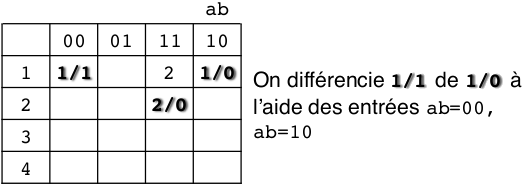
\includegraphics[width=.6\textwidth]{ch7/image43}
\end{figure}
Dans une machine de Meally, on peut à priori fusionner des états ayant des sorties différentes. La seule contrainte étant que l'on ne peut pas fusionner 2 états stables ayant la même combinaisons d'entrée (même colonne) \textbf{et} ayant une sortie différente
\begin{figure}[H]
	\centering
	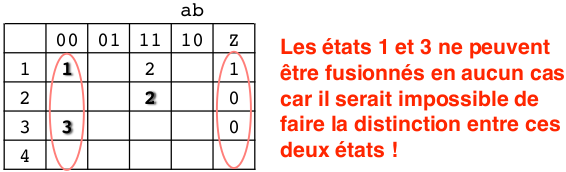
\includegraphics[width=.6\textwidth]{ch7/image44}
\end{figure}
\subsection{Synthèse de sortie}
Un peu plus compliqué car la sortie de l'état de départ dépend de l'entrée, du coup :
\begin{figure}[H]
	\centering
	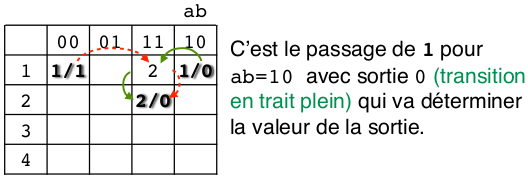
\includegraphics[width=.6\textwidth]{ch7/image45}
\end{figure}
Il faudra donc mettre obligatoirement un 0. C'est la seul subtilité, le reste ce fait exactement comme dans la \autoref{sec:synthfontsortie}
\subsection{Fusionnement}
Un petit exemple de fusionnement pour éviter toute ambiguïté
\begin{figure}[H]
	\centering
	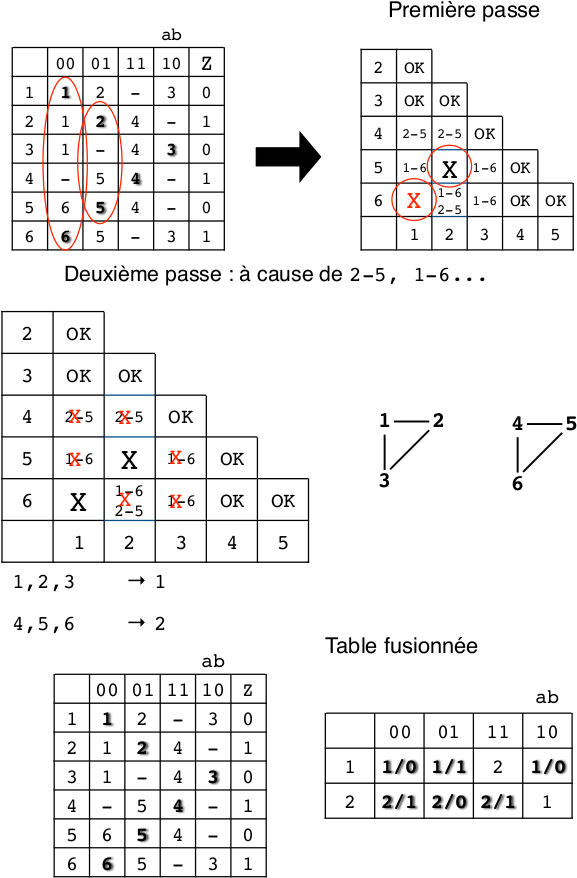
\includegraphics[width=.6\textwidth]{ch7/image46}
\end{figure}
\subsubsection{Fautes graves}
\begin{enumerate}
	\item Ne pas résoudre les transitions pour la fonction de sortie. Considérer la fonction de sortie comme uniquement fonction des variables d'état.
	\item Pour Meally, fusionner 2 états stables de la même colonne ayant des sorties différentes.
	\item  Faire une machine de Moore alors que l'on demandait Meally.
\end{enumerate}
\section{Aspects temporels des circuits séquentiels}
\subsection{Flip-flop D}
La spécificité est décrire dans la \autoref{subsec:Dflipflop}. On utilise ces flip-flops pour maîtriser les délais réels des portes logiques et des fils en ignorant les transitoire et ne regarder la sortie qu'au bon moment. On isole souvent un circuit logique par des flip-flops à l'entrée et à la sortie.
\begin{figure}[H]
	\centering
	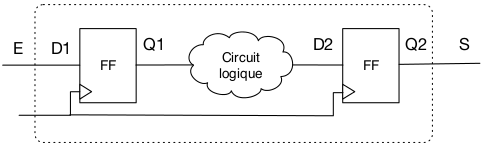
\includegraphics[width=.6\textwidth]{ch7/image47}
\end{figure}
Les conditions au bon fonctionnement du flip-flop est :
\begin{itemize}
	\item l'entrée D doit arrivée \textbf{avant} un certain temps - \emph{set-up time ($t_{su}$)}
	\item l'entrée D doit être maintenue \textbf{après} un certain temps - \emph{hold time ($t_h$)}
	\item dans cette fenêtre de temps, D \textbf{ne peut pas changer}
\end{itemize}
\begin{figure}[H]
	\centering
	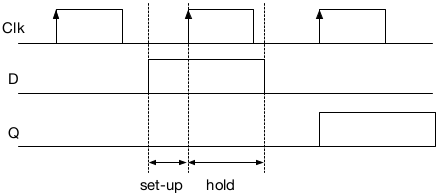
\includegraphics[width=.5\textwidth]{ch7/image48}
\end{figure}
Dans un circuit 
\begin{figure}[H]
	\centering
	\includegraphics[width=\textwidth]{ch7/image49}
\end{figure}
la réserve de temps ou \emph{slack} est :
\begin{itemize}
	\item positif : il y a une réserve de temps, possibilité de complexifier le circuit
	\item négatif : le circuit ne fonctionnera pas, pour résoudre ce problème :
	\begin{itemize}
		\item utiliser des portes plus rapide
		\item réduire le délai dans les fils
		\item augmenter la période
	\end{itemize}
\end{itemize}
le \emph{total negative slack} donne la mesure à quel point la contrainte est loin de la solution.\\

Pour les circuits complexes, on met en série des circuits logiques et des flip-flops pour résoudre les transitoires. La période des flip-flops dépendront de \textit{set-up}/\textit{hold time} et de la complexité du circuit.\\
Les données logiques transitent entre les flip-flops de manière synchrone car les flip-flops ont on la même référence temporelle (\textit{Register Transfer Logic} ou RTL).\\

L'autre avantage est le parallélisme des calculs (\textit{pipeline}). Pour un système à 2 circuits logiques combinatoire :
\begin{figure}[H] 
	\centering 
	\includegraphics[width=.8\textwidth]{ch7/image50} 
\end{figure}
\section{Moore ou Meally ?}
\begin{multicols}{2}
	\paragraph{Machine de Moore}
	\begin{itemize}
		\item Sortie valide aux états stables uniquement
		\item Sortie correcte au temps de transition prêt si nombre de transitions fixé à 1 seule
		\item Possible de tolérer ces délais
	\end{itemize}
	\columnbreak
	\paragraph{Machine de Meally}
	\begin{itemize}
		\item Sorties sensibles aux entrées !
		\item Peut être plus compacte en termes d'expressions logiques nécessaire pour produire les différents états du système
		\item Plus contraignante pour la fonction de sortie (moins de choix)
	\end{itemize}
\end{multicols}
Dans tous les  cas, ce sont toujours des systèmes \textbf{asynchrones} !\\

Une autre manière de résoudre les problèmes de transitions (et glitchs à la sortie) $\rightarrow$ ajouter des flip-flops.\\ \textbf{Synchronisation} des sorties : période d'horloge suffisamment longue pour permettre les transitions les plus longues, permettant d'ignorer les transitions (pour la sortie).
\begin{figure}[H] 
	\centering 
	\includegraphics[width=.7\textwidth]{ch7/image51} 
\end{figure}
\section{Circuits synchrones}
Le principe du circuit synchrone n'est pas de supprimer les courses critiques mais de mémoriser les variables d'états afin de solutionner ces courses. On va donc mettre à jour les variables par intervalles régulier (via une clock). Cette période sera suffisamment longue pour permettre la stabilisation des fonctions logiques de rétroaction.\\
Dire que $Y_i=f(E,y_i)$ ne signifie plus une égalité mais une affectation (\textit{CurrentState $\leftarrow$ NextState}).\\

Pour bien comprendre comment cela se passe : 
\begin{enumerate}
	\item on est dans l'état $00$ et on va passer à l'état $11$
	\begin{figure}[H] 
		\centering 
		\includegraphics[width=.3\textwidth]{ch7/image53} 
	\end{figure}
	\item Tant qu'il n'y a pas de mises à jour, les variables d'état du présent ne changent pas
	\item Toutes les variations à l'entrée de M est ignorée (les possibles états transitoires)
	\item Si la période de la clock est bien choisie, les transitoires se finissent avant le signal de synchronisation
	\item Le signal de synchronisation passe à 1 (ex. flanc montant d'un flip-flop) puis retourne à 0 
	\begin{figure}[H] 
		\centering 
		\includegraphics[width=.3\textwidth]{ch7/image54} 
	\end{figure}
	\item Le futur est devenu présent
	\item Le problème des courses entre les mémoire et les portes "du présent" na pas d'influence car tout transitoire à la sortie du CC est ignoré (le $y_1y_2=01$ provoque un transitoire pour $Y_1Y_2$ mais qui ne sera pas pris en compte, donc osef) 
\end{enumerate}
\subsection{Performance}
C'est clairement un nivellement vers le bas :
\begin{itemize}
	\item vitesse d'évolution fixée par la variable d'état la plus lente (les plus rapide devront attendre la plus lente)
\end{itemize}
Les systèmes asynchrones ont été évité car elles sont plus complexe à réalisée (nombre d'état grand) mais on commence a revenir sur nos pas pour des raisons de performance.

\subsection{Organe de mémoire = flip flop}
On peut utiliser des flip-flops (SR, JK, D et T) commandées par des fonctions logiques dérivées de la table d'état codée. Ces fonctions logiques de commande des flip-flops sont leurs \textbf{fonctions d'excitation}. La synthèse d'un circuit synchrone revient à faire la synthèse des fonctions d'excitation d'un organe de mémoire standard.
\begin{figure}[H] 
	\centering 
	\includegraphics[width=.6\textwidth]{ch7/image55} 
\end{figure}

\centerline{Différence entre asynchrone et synchrone}
\begin{multicols}{2}
	\paragraph{Asynchrone}
	\begin{itemize}
		\item Supprimer les courses critiques (\textit{C.f.} \autoref{subsec:resolcrit})
	\end{itemize}
	\columnbreak
	\paragraph{Synchrone}
	\begin{itemize}
		\item Laisser les courses critiques (codage arbitraire)
		\item Tables d'excitation
		\item fonctions d'excitation
	\end{itemize}
\end{multicols}
Le type d'organe de mémoire influence la complexité du circuit, mais ici on s'en fou, c'est imposé (on fournit la table d'état mais il faut savoir la dériver en table d'excitation).\\

\centerline{{\huge\danger}\ Lire à partir du slide 29 (cours 10) pour un exemple récapitulatif (de tout) ! {\huge\danger}}
\subsubsection{Fautes graves}
\begin{itemize}
	\item Ne pas savoir dériver les tables d'excitation pour les organes de mémoire
	\item Résoudre les courses critiques avant de dériver la table d'excitation de l'automate
	\item Établir la table d'excitation par rapport au entrées et pas par rapport aux variables d'état
\end{itemize}
\begin{figure}[H] 
	\centering 
	\includegraphics[width=.6\textwidth]{ch7/image52} 
	\caption{Table d'état $\rightarrow$ Table d'excitation}
\end{figure}
\begin{center}
	\textbf{\large Cours 11 chez soi}
\end{center}